% - Explain how data has been retrieved.

% - Data provider Energycharts(entsoe retrieves its data)

% - Explain the ETL(Extract Transform Load) pipeline
% I set up.

% - Explore data in order to get useful insights for
% how to tune the models to get the most of them.

% - correlation between temperatures and load, wind speeds and load


% - Split train and test dataset
% Explain carefully why it is important to carry
% out an out of sample test and not in sample.
% In sample test involves look ahead bias because we are
% fitting the model on the data we want to predict,
% thus it overfits on the data considered but it does
% not generalize well.

This section covers the datasets used in our experiments. In addition, attributes and features will be thoroughly described.
Next, we will explain the extract transform load pipeline (ETL) that we set up in order to ease the workflow of our studies.
Finally, in order to better understand patterns within the data, we carry out an exploratory data analysis.

\section{GEFCom2014}
The first class of datasets we identified are the ones from the GEFCom2014 competition. The data is freely hosted on Dr.\ Hong's blog \cite{hong2016probabilistic}.
The main reason is that, these datasets are considered an excellent test case for comparing predictive models between the EF community. Additionally, the scores of the competing models are freely available, this enables us to carry out a clean and transparent comparative study.
The GEFCom2014 consisted of four tracks: price, load, wind power and solar power forecasting. 
The GEFCom2014 folder contains a zip file for each of the four tracks.
We provide forecasts for the load and price quantities.
\\
\subsection{GEFCom2014 price track}
In the price forecasting track, the goal was to predict the electricity price for the next 24 hours of a single zone. 
The data can be found in the GEFCom2014-P\_V2 zip file alongside a set of instructions and the benchmark forecasts.
This data consists of time series for the locational marginal price, for the zonal load and for the system load. The data covers the time interval ranging from the $1^{st}$ of January 2011 to the $15^{th}$ of June 2013, see Figure \ref{fig:price_track_fig1}.\ 
Additionally, as the competition went on, the real observed data of the previous tasks were made available.
The 15 target days ordered by task number are: 16/06/2013, 17/06/2013, 24/06/2013, 04/07/2013, 09/07/2013, 13/07/2013, 16/07/2013, 18/07/2013, 19/07/2013, 20/07/2013, 24/07/2013, 25/07/2013, 07/12/2013, 08/12/2013, 17/12/2013. 
The first three tasks were designed for testing, they did not count for the competition.
\begin{figure}[!h]
    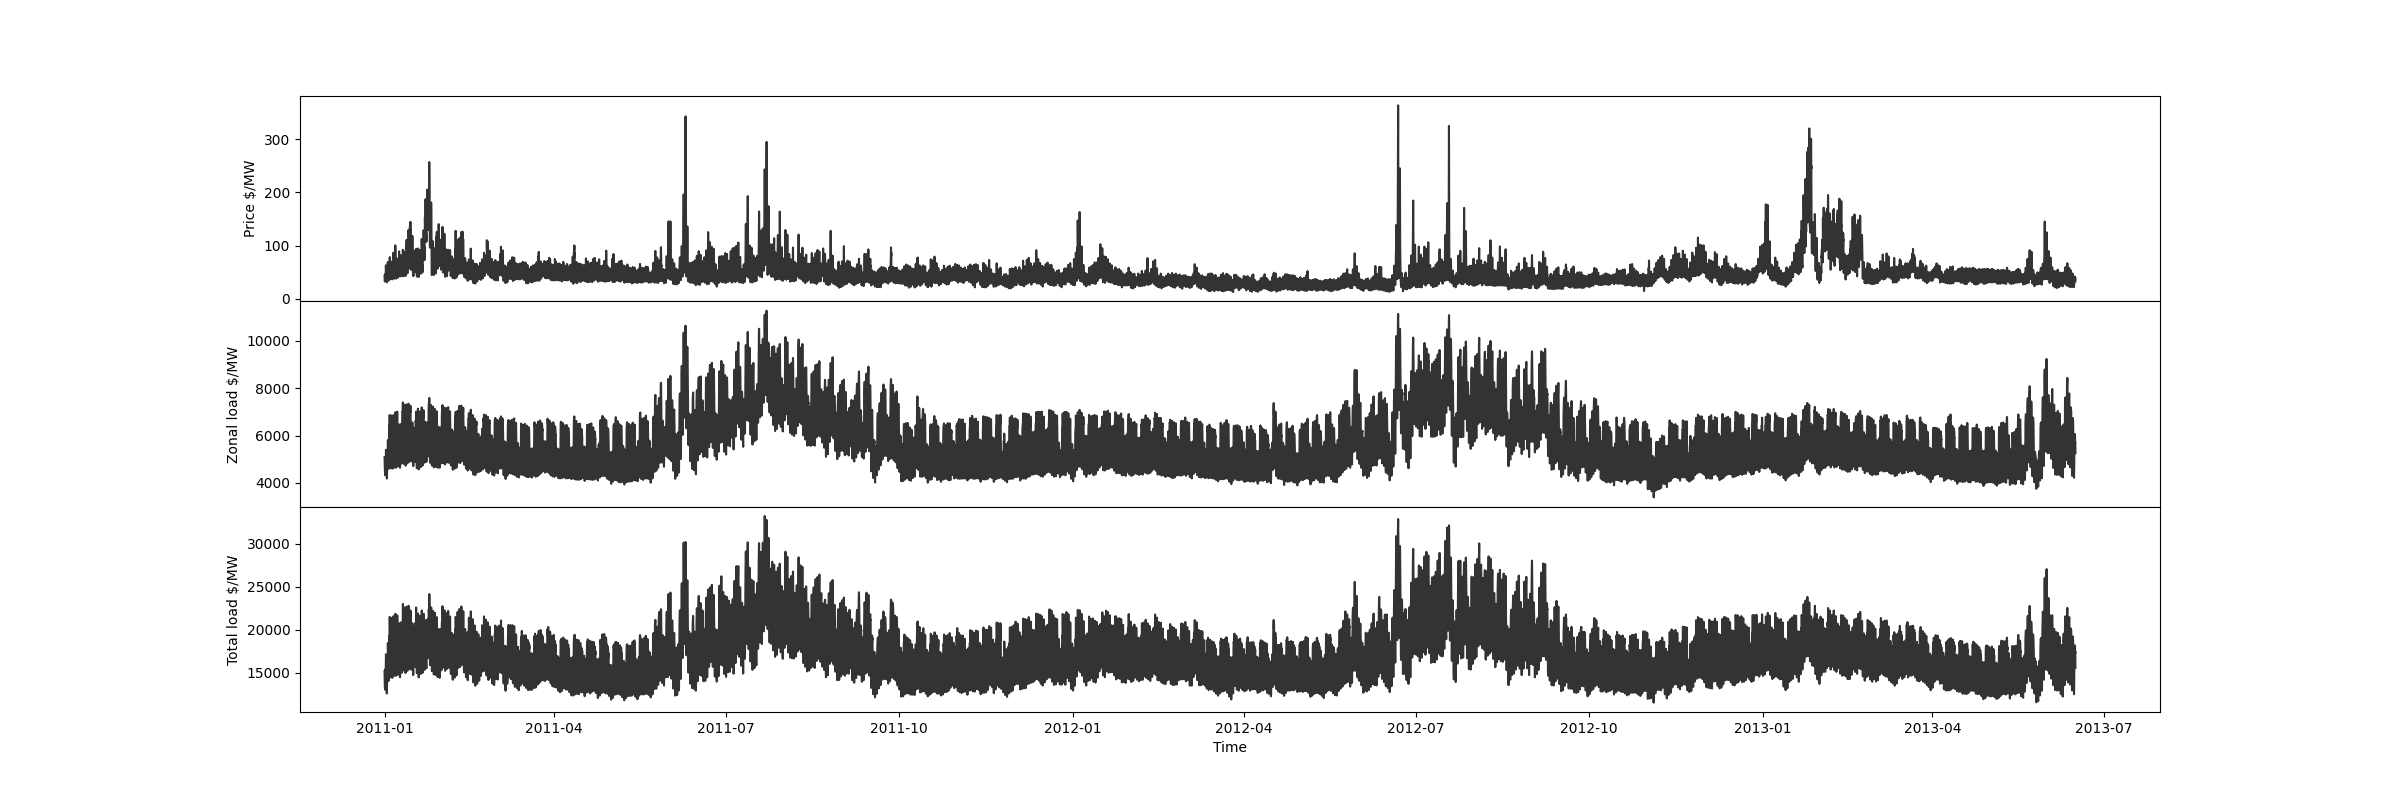
\includegraphics[width=\textwidth]{images/price_track_fig1.png}
    \caption{Price track GEFCom2014}
    \label{fig:price_track_fig1}
\end{figure}
\subsubsection{EDA}
In exploring this data we started off by plotting the time series of the zonal prices alongside with the total load and zonal load, see Figure \ref{fig:price_track_fig1}.
After that, we plotted the scatter plot for inspecting the correlation between the predictors and the dependent variables, Figure \ref{fig:gefcom_zonal_price_vs_zonal_load} and Figure \ref{fig:gefcom_zonal_price_vs_total_load}. From these visualisations, we can see their goodness for predicting zonal prices since there exists a clear correlation between the candidate predictors and the target variables.

\begin{figure}[!h]
    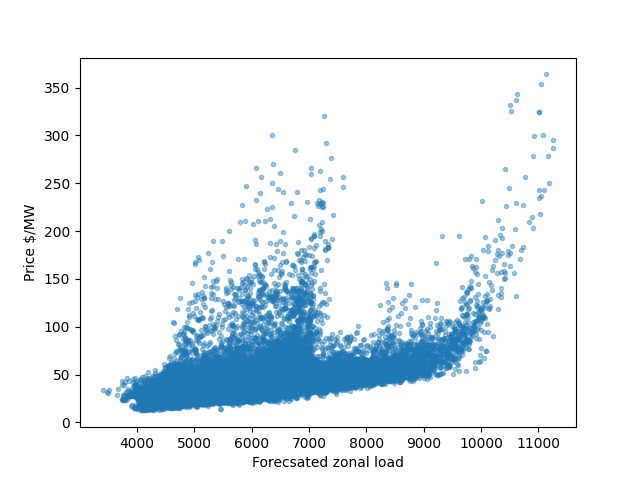
\includegraphics[width=\textwidth]{images/gefcom_zonal_price_vs_zonal_load.png}
    \caption{Zonal price versus zonal load of GEFCom2014}
    \label{fig:gefcom_zonal_price_vs_zonal_load}
\end{figure}


\begin{figure}[!h]
    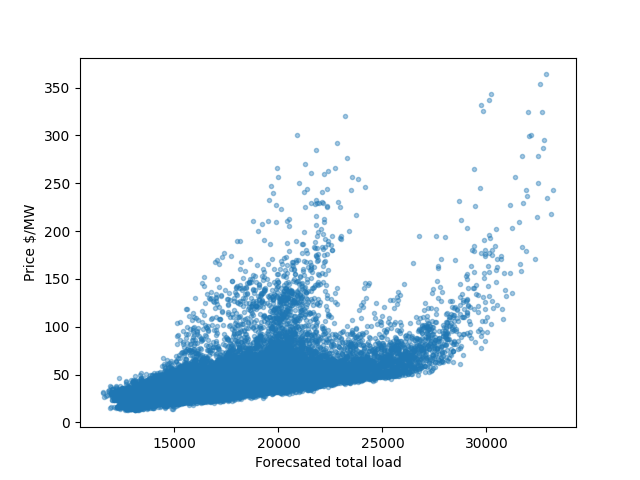
\includegraphics[width=\textwidth]{images/gefcom_zonal_price_vs_total_load.png}
    \caption{Zonal price versus total load of GEFCom2014}
    \label{fig:gefcom_zonal_price_vs_total_load}
\end{figure}

\subsection{GEFCom2014 load track}
In the load track, contestants were asked to provide one month ahead hourly probabilistic forecasts on a rolling basis for 15 consecutive rounds. To get started, in the first round, organizers provided 69 months of hourly load data (from 01/01/2005 to 30/10/2010) and 117 months of hourly temperature data (from 01/01/2001 to 30/10/2010). 
As for the price track, the true observed data from the previous track were made available as the competition progressed.
\\
The data for load forecasting is contained in the GEFCom2014-L\_V2 zip file. Within this subfolder, we have a txt file with the competition instructions and 15 subfolders one for each of the consecutive tasks. For each of those we have the prediction of the competition benchmark model and the train file upon which we will fit our model.
Any data from the various task folders are shifted by one month between each other.
Also in this track, the first three tasks do not count towards the ranking of the various algorithms.
\\
In order to compare our model performance with the winning entries of the GEFCom2014 load competition, we will refer to the Provisional\_Leaderboard\_\-V2.csv file contained also in the GEFCom2014 Data directory.
% Notice a quick premise, within this xsls file the authors opted for various scores to compare the entries performance. This choice was motivated by the need 
% to give a proportial weight to each task when averaging between them; that is in order to not penalise too much the tasks with higher point spreads. Furthermore, additional factors such as frequency of benchmark outperformance, and robustness and clarity in methodology explaination.
\\
The pinball scores for the load track are stored inside the subtab L-score-0/L-score-2 of Provisional\_Leaderboard\_V2.
\subsubsection{EDA}
We applied the same kind of EDA to the GEFCom load data. Figure \ref{fig:gefcom_load_historical} depicts the historical load while Figure \ref{fig:gefcom_w_avg_historical} reports the historical weather temperature. Finally, Figure \ref{fig:gefcom_load_vs_w_avg} shows the scatter plot between the load and the weather.
These plots motivate the selection of weather temperature as one of the predictors for the load.

\begin{figure}[!h]
    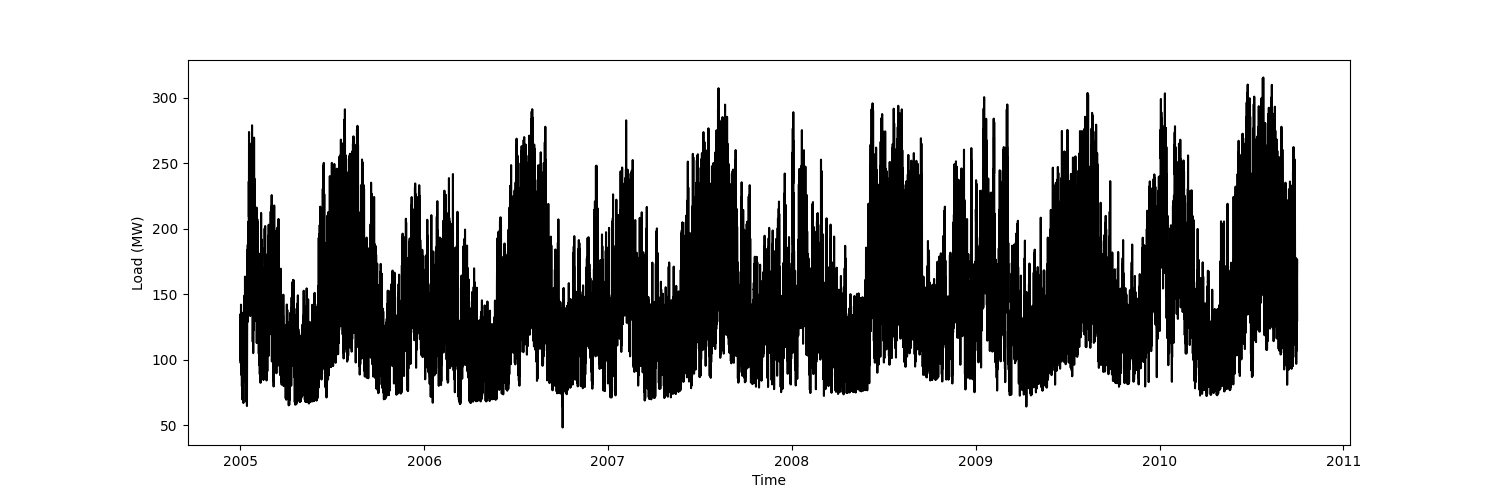
\includegraphics[width=\textwidth]{images/gefcom_load_historical.png}
    \caption{Historical load of GEFCom2014}
    \label{fig:gefcom_load_historical}
\end{figure}

\begin{figure}[!h]
    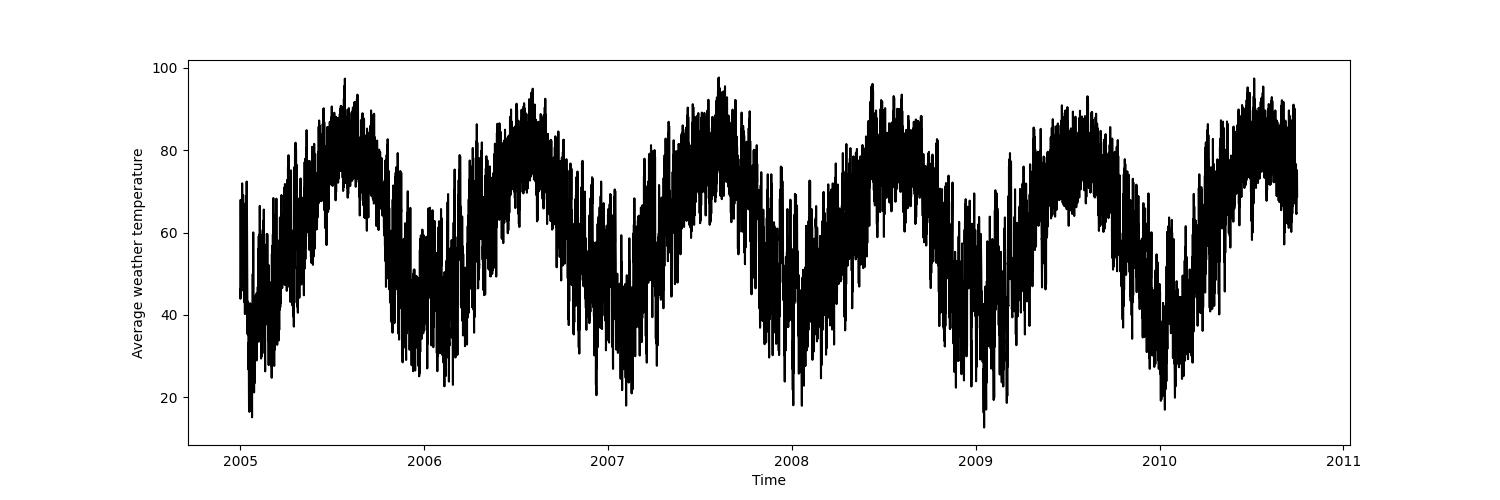
\includegraphics[width=\textwidth]{images/gefcom_w_avg_historical.png}
    \caption{Historical weather of GEFCom2014}
    \label{fig:gefcom_w_avg_historical}
\end{figure}

\begin{figure}[!h]
    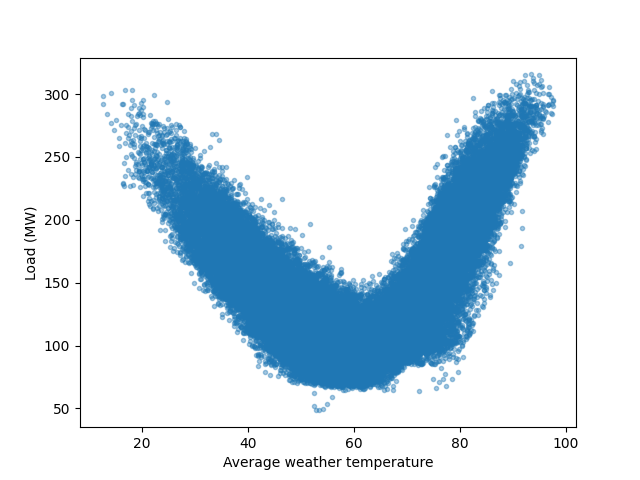
\includegraphics[width=\textwidth]{images/gefcom_load_vs_w_avg.png}
    \caption{Load versus weather of GEFCom2014}
    \label{fig:gefcom_load_vs_w_avg}
\end{figure}

% \subsection{GEFCom ETL}
\subsubsection{GEFCom ETL}
The provided data is raw, hence the need for a standardized extract transform and load pipeline. 
Firstly, we drop all Nans and zeros. The provided data for the challenge has a timestamp column not coherent to any time format. Thus, we first pass the data through a method extracting time information: hour, day, month and year. This info is then combined into a datetime object, we selected the ISO format.
Next, since the data does not provide the location for the target utility, the best we can do is selecting the average of weather temperatures as predictor variables. This independent variable is named w avg.
The same thing applies in the cleaning of the test data with the addition of an if clause for handling the different naming conventions and formatting used in the last track of the challenge. The Python ETL pipeline has since been automated to loop every task folder through Bash scripting.


\section{Germany Switzerland Austria data}
Next, we identified various data sources for Germany, Switzerland and Austria in order to further
investigate the techniques studied in this thesis.
Taking inspiration from the GEFCom2014 format, we firstly created a load track for Germany and Switzerland. 
The source of data has been the \href{https://www.energy-charts.info/index.html?l=en&c=DE}{energy charts} website. It provides data for electricity power, electricity potential capacity, energy generation, market prices, environmental measurements and also scenario simulations. This data is retrieved from the European network of transmission system operators for electricity \href{https://www.entsoe.eu/}{(ENTSOE)} and made available thanks to the \href{https://ise.fraunhofer.de/en.html}{Fraunhofer Institute for Solar Energy Systems ISE}.
\\
In this experiment, the goal is comparing kernel quantile regression to the other state of the art quantile regressors, see Section \ref{ch:prob}.
The target dependent variable is the national load while as predictors we took
the weather temperature, the wind speed, the date expressed in terms of the three attributes day, month and hour, a categorical variable for the day of the week and a binary categorical variable accounting for the holiday effect.


In the second experiment we compared various kernels in the context of load forecasting.
For this study, we considered the data of \href{https://zenodo.org/records/7907883}{SECURES-Met}. This data consists of various metereological attributes relevant for modelling electricity demand \cite{Formayer2023}. The dataset is made up of historical data until end of 2020, while from 2021 onwards the data consists of forecasts made by a metereological model developed by the European Centre for Medium-Range Weather Forecasts (ECMWF). The forecasted data is split in two files according to the scenarios RCP4.5 and RCP8.5. In our experiments, we considered the former. 
In this setting the independent variables available are 
direct irradiation, global radiation, power from reservoir plants, power from run of the river plants (ROR), weather temperature and wind potential.

\subsubsection{ETL}
From energy charts we downloaded the historical load along with the weather temperatures and wind speeds forecasts. The data request to the environmental variables at hourly frequency for a whole year is broken. Therefore, we downloaded each month separately and then transformed them into a single csv for the whole year.

For what concerns the data from SECURES-Met we first identified the data interesting to us. Next, we formatted all the csv to a coherent format, gave columns meaningful names, sliced for the years 2020 (train) and 2021 (test) and finally merged all single csv\textsubscript{s} together.

All the manipulations involved in the ETL pipeline have been carried out by combining Python and Bash scripting. 

\subsubsection{EDA}
Following we report the EDA plots alongside with insights that can be extracted from them. We choose to focus the following analysis on the Swiss data only, given that the plots for the German data are pretty similar.
To get started we visualise the historical load data in Figure \ref{fig:CH_historical_load_2021}. As expected, electricity load exhibits a seasonal pattern with highs in the winter and lows during the summer season.
\begin{figure}[!h]
    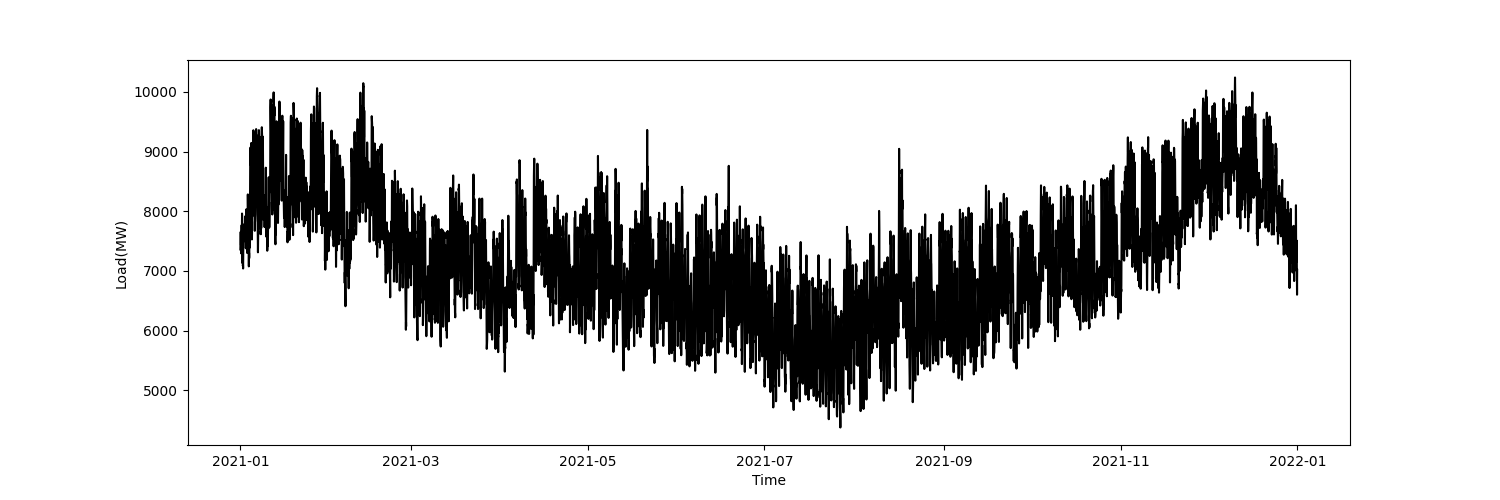
\includegraphics[width=\textwidth]{images/CH_historical_load_2021.png}
    \caption{Switzerland historical load (2021)}
    \label{fig:CH_historical_load_2021}
\end{figure}
Next, we built scatter plots of the independent continous variables against the load as means of visualizing correlation between them.
Figure \ref{fig:CH_load_vs_temperature_2021} plots load against temperatures while Figure \ref{fig:CH_load_vs_wind_speed_2021} depicts load against wind speed. From these plots, we can clearly see there exists a relationship that ties wind speeds and temperatures to load.

\begin{figure}[!h]
    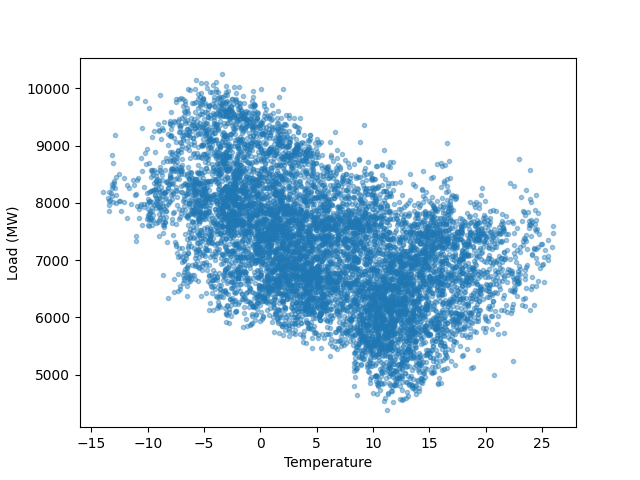
\includegraphics[width=\textwidth]{images/CH_load_vs_temperature_2021.png}
    \caption{Load versus temperature for Switzerland (2021)}
    \label{fig:CH_load_vs_temperature_2021}
\end{figure}

\begin{figure}[!h]
    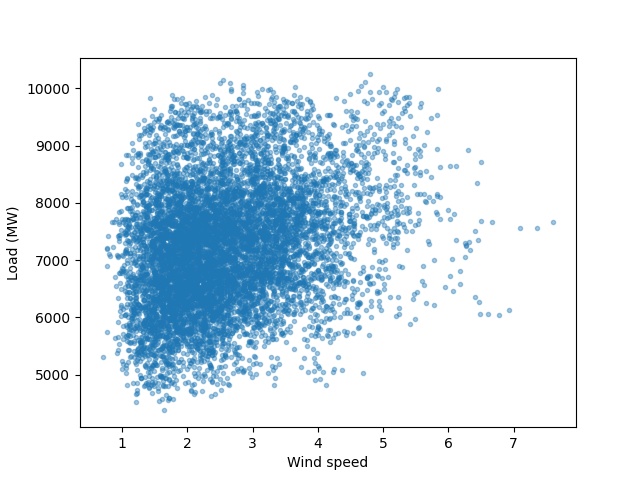
\includegraphics[width=\textwidth]{images/CH_load_vs_wind_speed_2021.png}
    \caption{Load versus wind speed for Switzerland (2021)}
    \label{fig:CH_load_vs_wind_speed_2021}
\end{figure}

Following, we use box plots in order to visualize the relations between categorical independent variables and the dependent one. Such visualisation are reported in Figure \ref{fig:CH_day_of_week_boxplot_2021} and Figure \ref{fig:CH_is_holiday_boxplot_2021}. We can see that workdays involve a higher load and possess a wider range than weekdays and holidays.

\begin{figure}[!h]
    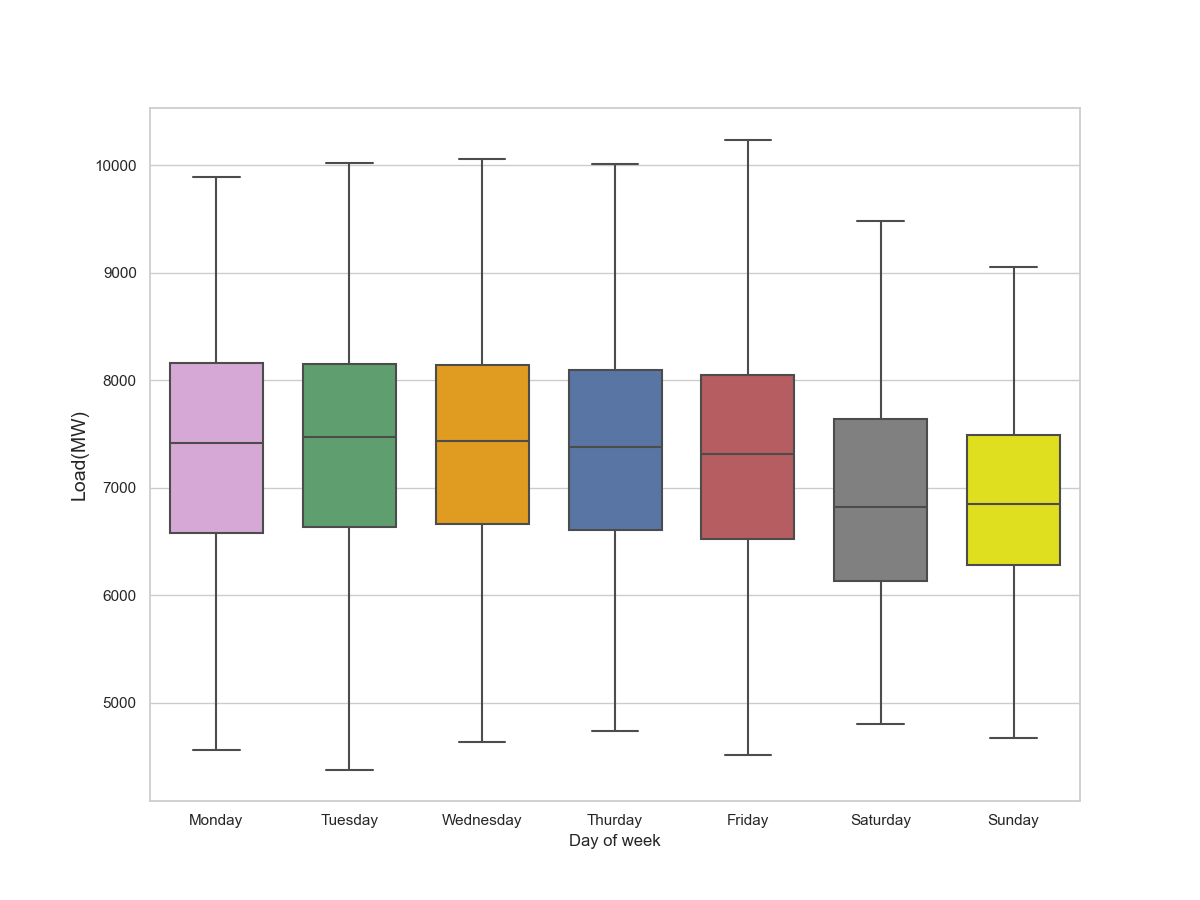
\includegraphics[width=\textwidth]{images/CH_day_of_week_boxplot_2021.png}
    \caption{Load versus day of week boxplot for Switzerland (2021)}
    \label{fig:CH_day_of_week_boxplot_2021}
\end{figure}

\begin{figure}[!h]
    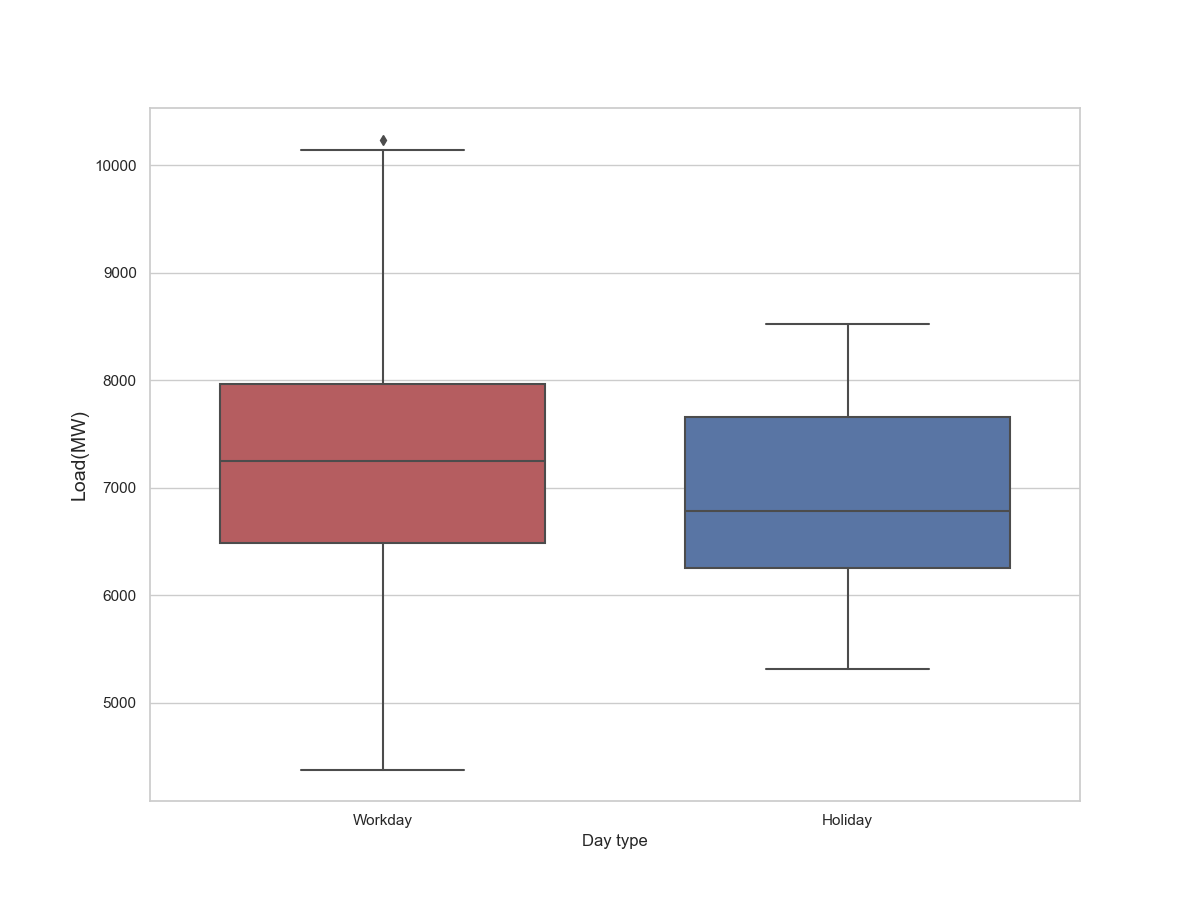
\includegraphics[width=\textwidth]{images/CH_is_holiday_boxplot_2021.png}
    \caption{Load versus day type boxplot for Switzerland (2021)}
    \label{fig:CH_is_holiday_boxplot_2021}
\end{figure}

We conclude this EDA by reporting the heatmap of independent variables alongside with the load in Figure \ref{fig:CH_heatmap_2021}. Temperature, wind speed and day of week show a meaningful correlation. This is a clear indication of their suitability as predictors for forecasting the load.

\begin{figure}[!h]
    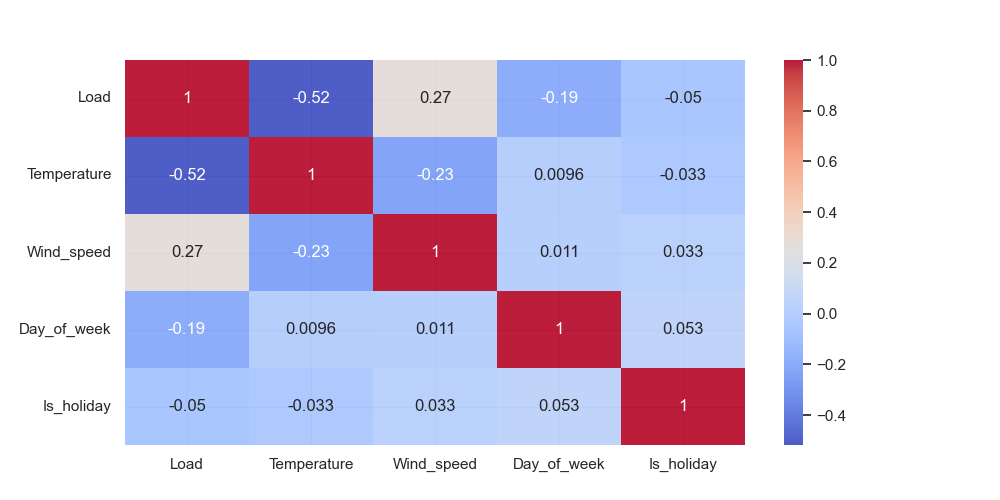
\includegraphics[width=\textwidth]{images/CH_heatmap_2021.png}
    \caption{Switzerland load heatmap (2021)}
    \label{fig:CH_heatmap_2021}
\end{figure}